\chapter{The Privacy Problem}
\label{ch:privacy-problem}

\begin{quote}
\textit{``Privacy is not about hiding wrongdoing. It's about protecting the ability to change and grow, to have different identities in different contexts, and to be free from the perfect memory of machines.''}
\end{quote}

You've seen how Bloom filters save space through approximation, and how hashing can transform data. Now we confront the real challenge: when you query a remote database, what does the server learn about you?

This chapter exposes the fundamental tension in information systems: functionality requires revelation. Every query you make, every pattern in your access, every correlation in your searches tells a story. We'll see why traditional approaches fail, setting the stage for our oblivious solution.

\section{What Privacy Means in Computing}

Privacy in computing isn't about encryption alone---encrypted data that reveals access patterns still leaks information. Consider three levels of privacy:

\begin{enumerate}
\item \textbf{Data Privacy}: The content itself is protected
\item \textbf{Access Privacy}: Which data you access is hidden  
\item \textbf{Pattern Privacy}: Statistical patterns in access are obscured
\end{enumerate}

Most systems stop at level 1. We're targeting level 3.

\subsection{The Observation Problem}

Every interaction with a system creates observations:

\begin{lstlisting}[language=Python]
# What the server sees
class ServerObservations:
    def log_query(self, query_hash, timestamp):
        # Even with hashed queries, patterns emerge
        self.query_log.append({
            'hash': query_hash,
            'time': timestamp,
            'source_ip': get_client_ip()
        })
    
    def analyze_patterns(self):
        # Frequency analysis
        freq = Counter(q['hash'] for q in self.query_log)
        
        # Temporal patterns  
        time_patterns = self.extract_time_patterns()
        
        # Correlation analysis
        correlations = self.find_query_pairs()
        
        return self.infer_user_interests(freq, time_patterns, correlations)
\end{lstlisting}

Even hashed queries leak information through:
\begin{itemize}
\item \textbf{Frequency}: Popular terms queried more often
\item \textbf{Timing}: Queries cluster around events
\item \textbf{Correlation}: Terms often searched together
\item \textbf{Volume}: Query rate reveals activity level
\end{itemize}

\section{Case Study: The Journalist's Dilemma}

Let's make this concrete with a running scenario that we'll revisit throughout the book.

\begin{example}[Investigative Journalism]
Sarah is investigating potential government corruption. She needs to search a document database for:
\begin{itemize}
\item Officials' names
\item Financial terms (``offshore'', ``payment'', ``transfer'')
\item Dates around key events
\item Connections between entities
\end{itemize}

Using a traditional search system, even with encryption:
\begin{lstlisting}[language=Python]
# Sarah's searches over one week
searches = [
    "senator_collins",           # Monday morning
    "offshore_accounts",          # Monday afternoon
    "senator_collins",           # Tuesday (checking again)
    "panama_papers",             # Wednesday
    "collins AND offshore",      # Thursday (correlation!)
    "transfer_2019_03",          # Friday (specific date)
]

# What adversary learns (even with hashing)
h1 = hash("senator_collins")    # Appears twice (high interest)
h2 = hash("offshore_accounts")   # Financial investigation
h3 = hash("panama_papers")       # Looking at leaks
# Correlation: h1 and h2 searched together (found connection!)
# Timeline: Specific date suggests transaction found
\end{lstlisting}

The server learns:
\begin{enumerate}
\item Sarah is investigating someone (repeated searches)
\item It involves offshore finances (topic clustering)
\item She found a connection (correlated search)
\item She's zeroing in on March 2019 (specific temporal focus)
\end{enumerate}
\end{example}

\section{Traditional Approaches and Their Failures}

\subsection{Approach 1: Trusted Third Party}

\textbf{Idea}: Route queries through a trusted proxy that hides the source.

\textbf{Problems}:
\begin{itemize}
\item Single point of failure
\item Proxy sees everything
\item Can be compromised or compelled
\item Doesn't hide patterns from database
\end{itemize}

\subsection{Approach 2: Homomorphic Encryption}

\textbf{Idea}: Compute on encrypted data without decrypting.

\begin{lstlisting}[language=Python]
# Conceptual homomorphic search
encrypted_query = homomorphic_encrypt("senator_collins")
encrypted_db = [homomorphic_encrypt(doc) for doc in database]
encrypted_results = search_on_encrypted(encrypted_query, encrypted_db)
results = homomorphic_decrypt(encrypted_results)
\end{lstlisting}

\textbf{Problems}:
\begin{itemize}
\item Computationally expensive (1000-1,000,000x slower)
\item Complex operations limited
\item Still reveals access patterns
\item Not practical for large databases
\end{itemize}

\subsection{Approach 3: Private Information Retrieval (PIR)}

\textbf{Idea}: Retrieve items without revealing which item.

\textbf{Problems}:
\begin{itemize}
\item Requires downloading entire database (information-theoretic PIR)
\item Or computational assumptions that may not hold (computational PIR)
\item Doesn't handle complex queries well
\item Scales poorly with database size
\end{itemize}

\subsection{Approach 4: Query Obfuscation}

\textbf{Idea}: Add fake queries to hide real ones.

\begin{lstlisting}[language=Python]
def obfuscate_query(real_query):
    fake_queries = generate_decoy_queries(n=10)
    all_queries = [real_query] + fake_queries
    random.shuffle(all_queries)
    
    results = []
    for query in all_queries:
        results.append(search(query))
    
    return results[all_queries.index(real_query)]
\end{lstlisting}

\textbf{Problems}:
\begin{itemize}
\item Bandwidth increased by factor of $n$
\item Fake queries must be indistinguishable
\item Statistical analysis can still identify patterns
\item Doesn't hide correlations well
\end{itemize}

\section{The Fundamental Tradeoffs}

Every privacy system faces three competing demands:

\begin{center}
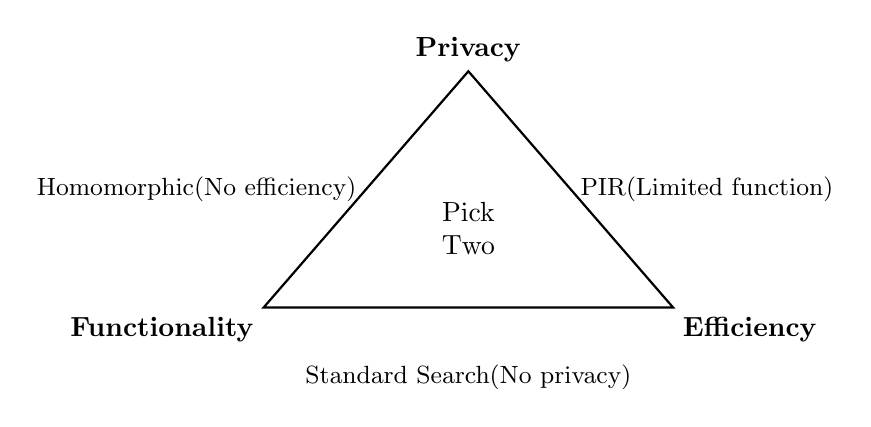
\begin{tikzpicture}[scale=2]
    % Triangle
    \coordinate (P) at (0,1.5);
    \coordinate (F) at (-1.3,0);
    \coordinate (E) at (1.3,0);
    
    % Draw triangle
    \draw[thick] (P) -- (F) -- (E) -- cycle;
    
    % Labels
    \node[above] at (P) {\textbf{Privacy}};
    \node[below left] at (F) {\textbf{Functionality}};
    \node[below right] at (E) {\textbf{Efficiency}};
    
    % Annotations
    \node[align=center] at (0,0.5) {Pick\\Two};
    
    % Examples on edges
    \node[left, font=\small] at (-0.65,0.75) {Homomorphic\\(No efficiency)};
    \node[right, font=\small] at (0.65,0.75) {PIR\\(Limited function)};
    \node[below, font=\small] at (0,-0.3) {Standard Search\\(No privacy)};
\end{tikzpicture}
\end{center}

Traditional approaches sacrifice one vertex:
\begin{itemize}
\item \textbf{High Privacy + Functionality} → Terrible efficiency (homomorphic)
\item \textbf{High Privacy + Efficiency} → Limited functionality (PIR)  
\item \textbf{High Functionality + Efficiency} → No privacy (standard)
\end{itemize}

\section{Information Leakage: A Formal View}

Let's formalize what privacy means using information theory.

\begin{definition}[Information Leakage]
Given a query $q$ and observations $O$, the information leakage is:
$$I(q; O) = H(q) - H(q|O)$$
where $H(q)$ is the entropy of queries and $H(q|O)$ is conditional entropy given observations.
\end{definition}

Perfect privacy requires $I(q; O) = 0$, meaning observations tell us nothing about queries.

\subsection{Sources of Leakage}

\begin{enumerate}
\item \textbf{Frequency Leakage}: 
   $$P(\text{query} = q | \text{observed } h) \propto P(h|q) \cdot P(q)$$
   More frequent terms are more likely given an observation.

\item \textbf{Correlation Leakage}:
   $$P(q_1, q_2 | \text{observed } h_1, h_2 \text{ together}) > P(q_1) \cdot P(q_2)$$
   Co-occurrence reveals relationships.

\item \textbf{Temporal Leakage}:
   $$P(q | \text{time pattern}) \neq P(q)$$
   Query timing reveals context.
\end{enumerate}

\subsection{The Distinguishability Problem}

An adversary wins if they can distinguish between query distributions:

\begin{lstlisting}[language=Python]
class PrivacyAdversary:
    def distinguish(self, observations):
        # Adversary's goal: Determine if observations come from
        # Distribution A (investigating corruption) or
        # Distribution B (routine research)
        
        features = self.extract_features(observations)
        # Frequency patterns
        # Correlation patterns  
        # Temporal patterns
        
        return self.classifier.predict(features)

# Privacy fails if:
# P(adversary_correct) > 0.5 + non_negligible
\end{lstlisting}

\section{Requirements for True Privacy}

Based on these failures, a truly private system must:

\begin{enumerate}
\item \textbf{Hide Access Patterns}: Which items are accessed must be obscured
\item \textbf{Provide Uniform Representations}: All queries should look identical
\item \textbf{Break Correlations}: Related queries shouldn't appear related
\item \textbf{Obscure Frequencies}: Common and rare queries indistinguishable
\item \textbf{Maintain Efficiency}: Still practical for real use
\item \textbf{Support Full Functionality}: Complex queries, updates, etc.
\end{enumerate}

This seems impossible! How can queries look identical yet return different results?

\section{The Bernoulli Insight}

Here's the key realization: \textit{approximate representations can provide exact privacy}.

Instead of making queries indistinguishable while preserving exact functionality (impossible), we:
\begin{enumerate}
\item Accept approximate results (Bloom filter style)
\item Make the approximations truly uniform
\item Hide all patterns in the noise
\end{enumerate}

\begin{proposition}[The Privacy-Approximation Exchange]
A system can achieve perfect observational privacy if:
\begin{enumerate}
\item All queries map to uniform random representations
\item Results are approximate with bounded error
\item Errors are independent of query content
\end{enumerate}
\end{proposition}

This leads to our framework:

\begin{center}
\begin{tikzpicture}
    % Input
    \node[draw, rectangle] (input) at (0,0) {True Query $q$};
    
    % Encoding
    \node[draw, rectangle, fill=blue!20] (encode) at (3,0) {Bernoulli\\Encode};
    \draw[->] (input) -- (encode);
    
    % Oblivious representation
    \node[draw, rectangle, fill=red!20] (oblivious) at (6,0) {Uniform\\Noise $\tilde{q}$};
    \draw[->] (encode) -- (oblivious);
    
    % Server processing
    \node[draw, rectangle] (server) at (9,0) {Server\\Process};
    \draw[->] (oblivious) -- (server);
    
    % Results
    \node[draw, rectangle, fill=red!20] (results) at (9,-2) {Noisy\\Results $\tilde{r}$};
    \draw[->] (server) -- (results);
    
    % Decoding
    \node[draw, rectangle, fill=blue!20] (decode) at (6,-2) {Bernoulli\\Decode};
    \draw[->] (results) -- (decode);
    
    % Output
    \node[draw, rectangle] (output) at (3,-2) {Approximate\\Results $r'$};
    \draw[->] (decode) -- (output);
    
    % Adversary
    \node[draw, ellipse, fill=gray!30] (adversary) at (7.5,1.5) {Adversary};
    \draw[dashed, ->] (oblivious) -- (adversary);
    \draw[dashed, ->] (server) -- (adversary);
    \node[right] at (9,1.5) {Sees only uniform noise!};
\end{tikzpicture}
\end{center}

\section{Preview: The Solution Architecture}

Our solution combines three key ideas:

\subsection{1. Bernoulli Types (Approximation)}
Replace exact data structures with probabilistic ones:
\begin{itemize}
\item Sets → Bloom filters (false positives)
\item Maps → Bernoulli maps (value uncertainty)
\item Numbers → Bernoulli floats (bounded error)
\end{itemize}

\subsection{2. Oblivious Encoding (Uniformity)}
Transform operations to look identical:
\begin{itemize}
\item All queries → Fixed-size bit vectors
\item All operations → Same computation pattern
\item All results → Indistinguishable noise
\end{itemize}

\subsection{3. Correlation Breaking (Independence)}
Hide relationships between queries:
\begin{itemize}
\item Tuple encoding for common pairs
\item Frequency normalization
\item Temporal shuffling
\end{itemize}

\section{What We Sacrifice and Gain}

\subsection{We Sacrifice}
\begin{itemize}
\item \textbf{Perfect Accuracy}: Results have bounded error (e.g., 0.1\% false positives)
\item \textbf{Some Space}: Oblivious structures larger than exact ones
\item \textbf{Query Precision}: Can't distinguish very similar items perfectly
\end{itemize}

\subsection{We Gain}
\begin{itemize}
\item \textbf{True Privacy}: Observations reveal nothing
\item \textbf{Practical Performance}: 10-100x faster than homomorphic
\item \textbf{Full Functionality}: Boolean queries, updates, ranking
\item \textbf{Provable Security}: Information-theoretic guarantees
\end{itemize}

\section{The Road Ahead}

In the next chapter, we'll build our first oblivious system, transforming the vulnerable search from our journalist example into one where Sarah can investigate without fear of observation.

The key insight to carry forward: \textit{by embracing approximation, we can achieve what exact computation cannot---true privacy in practical systems}.

\begin{inpractice}
Real-world systems using these ideas include:
\begin{itemize}
\item Private contact discovery (Signal)
\item Anonymous credentials (Privacy Pass)
\item Private set intersection (Apple/Google contact tracing)
\item Oblivious DNS (Cloudflare)
\end{itemize}

Each makes the same trade: accept small errors for strong privacy.
\end{inpractice}

\section{Exercises}

\begin{enumerate}
\item \textbf{Leakage Analysis}: Given a log of hashed queries, what can you infer about user interests using only frequency analysis?

\item \textbf{Correlation Detection}: If queries ``encryption'' and ``backdoor'' appear together 5x more often than expected by independence, what might this suggest?

\item \textbf{Privacy Metrics}: Calculate the information leakage $I(q; O)$ for a system where each query appears with frequency $p_i$ and is observed with probability $p_i^2$.

\item \textbf{Tradeoff Exploration}: For your favorite application, identify which vertex of the privacy-functionality-efficiency triangle you'd sacrifice and why.

\item \textbf{Attack Simulation}: Write code to distinguish between random queries and queries following a theme (e.g., medical research vs. financial investigation).
\end{enumerate}

\section{Further Reading}

\begin{itemize}
\item Goldreich \& Ostrovsky (1996): Software protection and simulation on oblivious RAMs
\item Gentry (2009): Fully homomorphic encryption
\item Islam et al. (2012): Access pattern disclosure attacks
\item Cash et al. (2015): Leakage-abuse attacks
\item Patel et al. (2019): Private information retrieval survey
\end{itemize}

\section{Chapter Summary}

Privacy in computing isn't just about hiding data---it's about hiding access patterns, correlations, and frequencies. Traditional approaches fail because they try to preserve exact functionality while achieving privacy, hitting fundamental impossibility results.

Our insight: approximate data structures that introduce controlled errors can achieve perfect observational privacy. By making all queries look like uniform random noise, we hide not just what you're searching for, but that you're searching at all.

Next, we'll build this vision into reality, creating your first oblivious system that provides true privacy through the power of probabilistic approximation.